% =====================================================================
%  Guía de laboratorio — IEL04 — Circuitos Eléctricos I, semana 6
%  Escrita por src/guia_laboratorio.py con la plantilla institucional
%  (config/framework_iub/guia-laboratorio/: guialabiub.sty e img/, copiados a esta carpeta).
%
%  Compilar con:  pdflatex -> biber -> pdflatex -> pdflatex
%  (En Overleaf: compilador pdfLaTeX; biber se ejecuta solo.)
% =====================================================================
\documentclass[12pt]{article}

% Opciones: [sinmarca] quita la marca de agua; [borrador] muestra márgenes
%           [ieee] referencias IEEE (por defecto); [apa] referencias APA 7
\usepackage{guialabiub}

% --------------------- Diagramas de flujo del procedimiento ----------------
% (TikZ, con los mismos estilos del .tex del temario; la plantilla no los trae)
\usepackage{tikz}
\usetikzlibrary{arrows.meta,positioning,shapes.geometric,shapes.misc}
\usepackage{adjustbox}
\definecolor{iubnavy}{HTML}{121023}
\definecolor{iubyellow}{HTML}{FFDF2D}
\definecolor{iubblue}{HTML}{00ADE7}
\definecolor{iuborange}{HTML}{E39037}
\definecolor{iubgreen}{HTML}{3B9C6D}
\definecolor{iubpurple}{HTML}{8E6BBF}
\definecolor{iubgris}{HTML}{D5DAE3}
\definecolor{iubgrisoscuro}{HTML}{7C8598}
\definecolor{iubfondoazul}{HTML}{EBF7FD}
\definecolor{iubfondonaranja}{HTML}{FDF4EA}
\definecolor{iubfondoverde}{HTML}{EDF8F2}
\definecolor{iubfondogris}{HTML}{F4F6F9}
\tikzset{
  dcaja/.style={draw=iubblue, fill=iubfondoazul, line width=1pt, rounded corners=1pt, align=center, inner sep=2pt},
  destado/.style={draw=iubblue, fill=iubfondoazul, line width=1pt, rounded corners=6pt, align=center, inner sep=2pt},
  ddecision/.style={draw=iuborange, fill=iubfondonaranja, line width=1pt, diamond, aspect=1.6, align=center, inner sep=1pt},
  dterminal/.style={draw=iubgreen, fill=iubfondoverde, line width=1pt, rounded rectangle, align=center, inner sep=2pt},
  dflecha/.style={-{Stealth[length=2.4mm]}, line width=0.9pt, draw=iubnavy},
  drotulo/.style={font=\footnotesize, text=iubgrisoscuro, fill=white, fill opacity=0.92, text opacity=1, inner sep=1.5pt},
}

% --------------------------- Bibliografía ----------------------------
\addbibresource{IEL04-semana06.bib}

% --------------------------- Datos de la guía -------------------------
\facultad{Facultad de Ingenierías}
\modulo{IEL04 --- Circuitos Eléctricos I}
\docente{Ing. Sergio Martinez Castilla}

\begin{document}

% Orden de la bibliografía: el mismo del .md (biblatex numera por orden de primera cita)
\nocite{ref1,ref2,ref3}

\datosguia
\lineablanco

% Título de la práctica y ficha de la sesión
{\centering\bfseries Guía de laboratorio: Circuito RC en paralelo: corrientes de rama, corriente total y ley de corrientes de Kirchhoff\par}
\lineablanco
\textbf{Semana:} 6 de 14 \quad \textbf{Resultado de aprendizaje:} IEL04-RA2 \quad \textbf{Práctica:} propuesta a partir de la bibliografía \cite{ref1}, \cite{ref2}, \cite{ref3} \quad \textbf{Duración:} \SI{240}{\minute}
\lineablanco
La práctica corresponde a la sesión teórica de la semana 6, \guillemotleft{}El circuito RC en paralelo: admitancia, reparto de corrientes y ley de corrientes de Kirchhoff\guillemotright{}, y reproduce su caso de estudio con los mismos componentes de la semana 4 conectados en paralelo: se miden a 1 kHz la corriente de cada rama y la corriente total, y se comprueba que la corriente total es la suma fasorial de las corrientes de rama. No hay un manual de laboratorio asignado al RA IEL04-RA2, por lo que la práctica se propone a partir de la bibliografía cargada: Floyd trata la admitancia y el análisis de circuitos RC en paralelo y la ley de corrientes de Kirchhoff \cite{ref1}, Boylestad las redes de ca en paralelo \cite{ref2} y Deorsola las leyes de Kirchhoff con fasores \cite{ref3}.

% ---------------------------------------------------------------------
\section{Objetivos}\label{sec:objetivos}
\textbf{Objetivo general:} Verificar experimentalmente la ley de corrientes de Kirchhoff y el ángulo de fase en un circuito RC en paralelo.
\lineablanco
\textbf{Objetivos específicos:}
\begin{itemize}
  \item Identificar y verificar con instrumentos el resistor y el condensador del circuito. \emph{(CE1)}
  \item Medir con el multímetro la corriente de la rama resistiva y la de la rama capacitiva a 1 kHz. \emph{(CE2)}
  \item Medir la corriente total y su desfase respecto de la tensión, y comprobar la suma fasorial de las corrientes de rama en el circuito RC en paralelo. \emph{(CE3)}
\end{itemize}

% ---------------------------------------------------------------------
\section{Materiales y Equipos}\label{sec:materiales}
\begin{itemize}
  \item \textbf{Resistor de película}: 1,5 k\ensuremath{\Omega} \textpm{}5 \%
  \item \textbf{Condensador C2 del kit}: 104K, 97,8 nF medidos
  \item \textbf{Resistor sensor de corriente}: 10 \ensuremath{\Omega}
  \item \textbf{Generador de funciones}
  \item \textbf{Osciloscopio de dos canales con puntas \texttimes{}10}
  \item \textbf{Multímetro digital de verdadero valor eficaz} (2)
  \item \textbf{Medidor LCR}
  \item \textbf{Protoboard}
  \item \textbf{Cables de conexión} (12)
  \item \textbf{Resistencia de descarga}: 1 k\ensuremath{\Omega}
\end{itemize}

% ---------------------------------------------------------------------
\section{Procedimiento}\label{sec:procedimiento}
La práctica ocupa el bloque de 2 h de laboratorio de la sesión y se realiza en grupos de tres estudiantes, con tres roles que rotan entre etapas: quien monta y opera el circuito, quien mide y quien registra y verifica los cálculos. Antes de energizar cualquier montaje, el docente o el monitor revisa la conexión. Cada etapa abre con su diagrama de flujo, que muestra la secuencia y las comprobaciones de un vistazo, y sigue con sus pasos numerados; cada paso indica cuánto dura, qué debe observarse para saber que salió bien y qué hacer si no. Los valores numéricos de la sesión teórica sirven de referencia: las lecturas propias del grupo se registran en las tablas de la sección de análisis.
\lineablanco
% --- Etapa 1: Preparación y montaje (3 pasos) ---
\subsection{Preparación y montaje (\SI{16}{\minute})}\label{sec:etapa-1}
% --- Figura 1: diagrama de flujo de la etapa 1 (TikZ; misma disposición que el PNG del .md) ---
\begin{figure}[H]
  \centering
\begin{adjustbox}{max width=\linewidth}
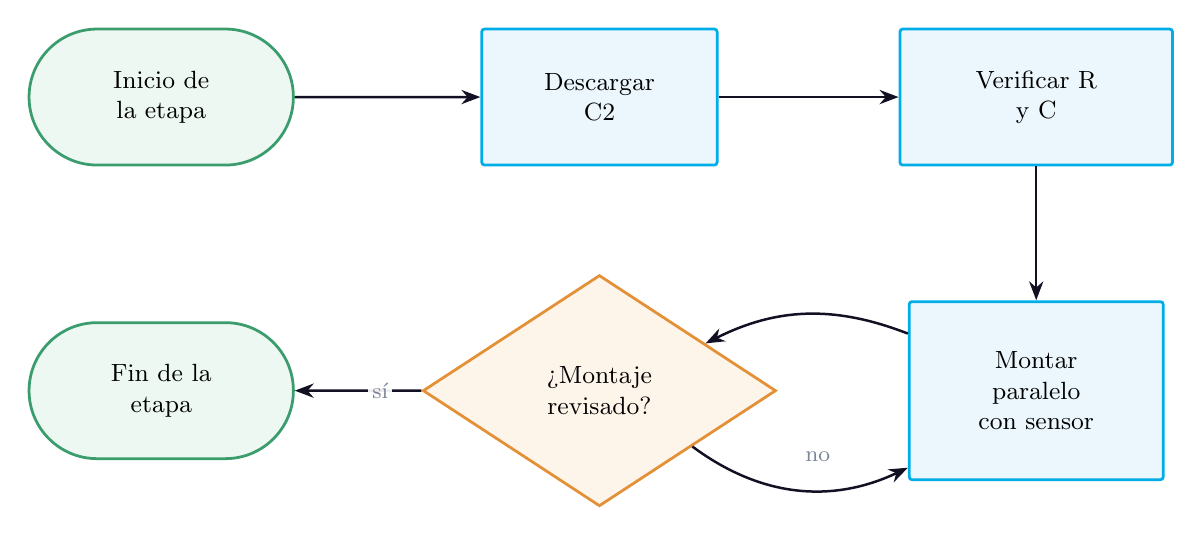
\begin{tikzpicture}[x=1in, y=1in, font=\small]
  % nodos (centro en pulgadas, con el tamano que calcula figuras.py)
  \node[dterminal, minimum width=1.377in, minimum height=0.680in] (n0) at (0.689,-0.340) {Inicio de \\ la etapa};  % ini
  \node[dcaja, minimum width=1.177in, minimum height=0.680in] (n1) at (2.880,-0.340) {Descargar \\ C2};  % a0
  \node[dcaja, minimum width=1.363in, minimum height=0.680in] (n2) at (5.064,-0.340) {Verificar R \\ y C};  % a1
  \node[dcaja, minimum width=1.270in, minimum height=0.890in] (n3) at (5.064,-1.808) {Montar \\ paralelo \\ con sensor};  % a2
  \node[ddecision, minimum width=1.766in, minimum height=1.156in] (n4) at (2.880,-1.808) {\textquestiondown{}Montaje \\ revisado?};  % dec
  \node[dterminal, minimum width=1.377in, minimum height=0.680in] (n5) at (0.689,-1.808) {Fin de la \\ etapa};  % fin
  % flechas (las de retorno, curvas)
  \draw[dflecha] (n0) -- (n1);
  \draw[dflecha] (n1) -- (n2);
  \draw[dflecha] (n2) -- (n3);
  \draw[dflecha] (n3) to[bend right=24] (n4);
  \draw[dflecha] (n4) -- (n5);
  \draw[dflecha] (n4) to[bend right=31] (n3);
  % rotulos de las flechas (donde los pone el PNG: sin caer sobre un nodo)
  \node[drotulo] at (1.784,-1.808) {sí};
  \node[drotulo] at (3.972,-2.136) {no};
\end{tikzpicture}
\end{adjustbox}
  \caption{Diagrama de flujo de la etapa 1: Preparación y montaje}
  \label{fig:flujo-1}
\end{figure}
\begin{pasos}
  \item \textbf{Paso~1:} Descargar el condensador conectando entre sus terminales, durante unos segundos, una resistencia de 1 k\ensuremath{\Omega} sujeta con pinzas aisladas, y medir con el voltímetro en cd la tensión entre terminales. \emph{(aprox.~\SI{3}{\minute})} \textbf{Comprobación:} La tensión debe ser prácticamente nula (menos de 0,1 V); si no lo es, repetir la descarga antes de manipular el componente. \textbf{Seguridad:} No cortocircuitar los terminales con los dedos ni con una herramienta metálica: un condensador puede conservar carga después de desconectado.
  \item \textbf{Paso~2:} Verificar el resistor con el ohmímetro y el condensador C2 con el medidor LCR, y anotar sus valores medidos. \emph{(aprox.~\SI{6}{\minute})} \textbf{Comprobación:} El resistor debe leer cerca de 1492 \ensuremath{\Omega} y C2 cerca de 97,8 nF; si alguno sale de su tolerancia, reemplazarlo y anotar el nuevo valor.
  \item \textbf{Paso~3:} Montar el resistor y C2 en paralelo y dejar en serie con la fuente el resistor sensor de 10 \ensuremath{\Omega}, del lado de tierra, para observar la forma de onda de la corriente total. \emph{(aprox.~\SI{7}{\minute})} \textbf{Comprobación:} El docente revisa el montaje; el sensor debe quedar entre el paralelo y la tierra del generador. \textbf{Seguridad:} Montar con el generador apagado.
\end{pasos}
% --- Etapa 2: Medición de las corrientes (4 pasos) ---
\subsection{Medición de las corrientes (\SI{30}{\minute})}\label{sec:etapa-2}
% --- Figura 2: diagrama de flujo de la etapa 2 (TikZ; misma disposición que el PNG del .md) ---
\begin{figure}[H]
  \centering
\begin{adjustbox}{max width=\linewidth}
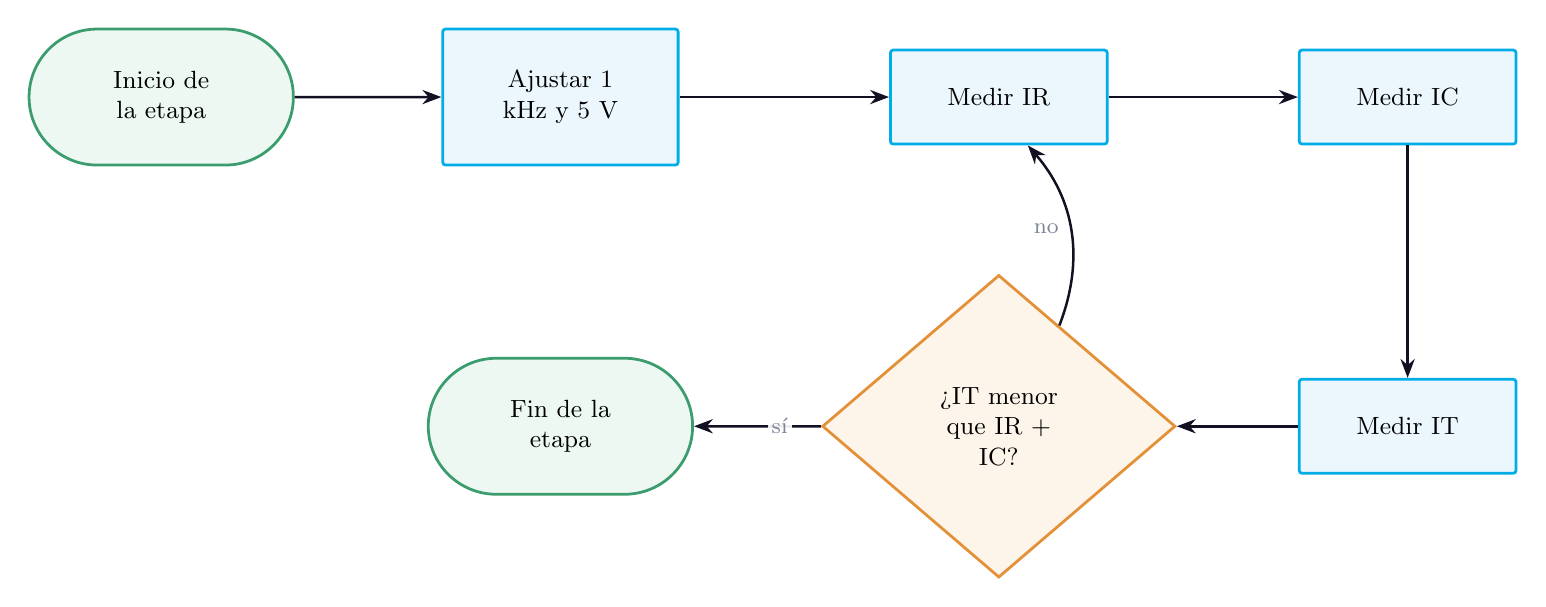
\begin{tikzpicture}[x=1in, y=1in, font=\small]
  % nodos (centro en pulgadas, con el tamano que calcula figuras.py)
  \node[dterminal, minimum width=1.377in, minimum height=0.680in] (n0) at (0.689,-0.340) {Inicio de \\ la etapa};  % ini
  \node[dcaja, minimum width=1.177in, minimum height=0.680in] (n1) at (2.685,-0.340) {Ajustar 1 \\ kHz y 5 V};  % a0
  \node[dcaja, minimum width=1.084in, minimum height=0.470in] (n2) at (4.877,-0.340) {Medir IR};  % a1
  \node[dcaja, minimum width=1.084in, minimum height=0.470in] (n3) at (6.921,-0.340) {Medir IC};  % a2
  \node[dcaja, minimum width=1.084in, minimum height=0.470in] (n4) at (6.921,-1.986) {Medir IT};  % a3
  \node[ddecision, minimum width=1.766in, minimum height=1.513in] (n5) at (4.877,-1.986) {\textquestiondown{}IT menor \\ que IR + \\ IC?};  % dec
  \node[dterminal, minimum width=1.377in, minimum height=0.680in] (n6) at (2.685,-1.986) {Fin de la \\ etapa};  % fin
  % flechas (las de retorno, curvas)
  \draw[dflecha] (n0) -- (n1);
  \draw[dflecha] (n1) -- (n2);
  \draw[dflecha] (n2) -- (n3);
  \draw[dflecha] (n3) -- (n4);
  \draw[dflecha] (n4) -- (n5);
  \draw[dflecha] (n5) -- (n6);
  \draw[dflecha] (n5) to[bend right=31] (n2);
  % rotulos de las flechas (donde los pone el PNG: sin caer sobre un nodo)
  \node[drotulo] at (3.781,-1.986) {sí};
  \node[drotulo] at (5.114,-0.999) {no};
\end{tikzpicture}
\end{adjustbox}
  \caption{Diagrama de flujo de la etapa 2: Medición de las corrientes}
  \label{fig:flujo-2}
\end{figure}
\begin{pasos}
  \item \textbf{Paso~4:} Ajustar el generador a una onda sinusoidal de 1 kHz y medir con el osciloscopio y con el multímetro de verdadero valor eficaz que la tensión en los bornes del circuito, con el circuito conectado, sea de 5,00 V eficaces. \emph{(aprox.~\SI{6}{\minute})} \textbf{Comprobación:} El multímetro debe indicar 5,00 V y el osciloscopio una sinusoide sin distorsión; si la tensión baja al conectar el circuito, reajustar la amplitud con el circuito conectado.
  \item \textbf{Paso~5:} Con el circuito desenergizado, insertar el multímetro en serie con la rama del resistor, energizar y anotar la corriente $I_R$. \emph{(aprox.~\SI{8}{\minute})} \textbf{Comprobación:} Debe leerse cerca de 3,35 mA; si la lectura es nula, revisar que el multímetro esté en la función de corriente alterna. \textbf{Seguridad:} Insertar el amperímetro solo con el circuito desenergizado.
  \item \textbf{Paso~6:} Repetir en la rama del condensador y anotar $I_C$. \emph{(aprox.~\SI{8}{\minute})} \textbf{Comprobación:} Debe leerse cerca de 3,07 mA.
  \item \textbf{Paso~7:} Repetir en serie con la fuente y anotar la corriente total $I_T$. \emph{(aprox.~\SI{8}{\minute})} \textbf{Comprobación:} Debe leerse cerca de 4,55 mA, menor que la suma aritmética de las ramas; si coincide con la suma, revisar las conexiones.
\end{pasos}
% --- Etapa 3: Ángulo de fase de la corriente total (3 pasos) ---
\subsection{Ángulo de fase de la corriente total (\SI{19}{\minute})}\label{sec:etapa-3}
% --- Figura 3: diagrama de flujo de la etapa 3 (TikZ; misma disposición que el PNG del .md) ---
\begin{figure}[H]
  \centering
\begin{adjustbox}{max width=\linewidth}
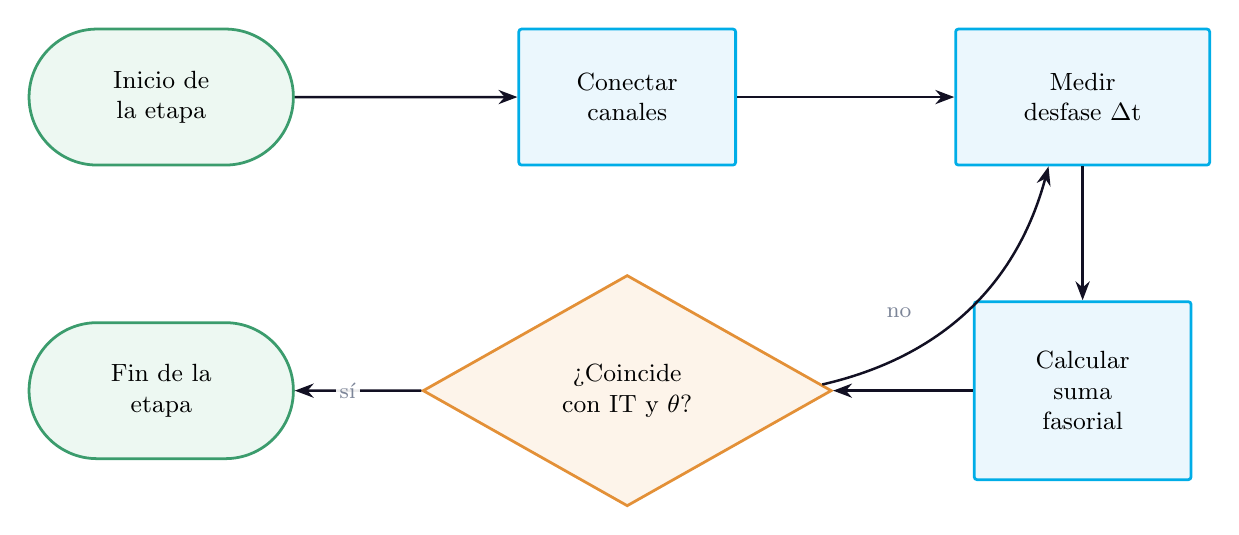
\begin{tikzpicture}[x=1in, y=1in, font=\small]
  % nodos (centro en pulgadas, con el tamano que calcula figuras.py)
  \node[dterminal, minimum width=1.377in, minimum height=0.680in] (n0) at (0.689,-0.340) {Inicio de \\ la etapa};  % ini
  \node[dcaja, minimum width=1.084in, minimum height=0.680in] (n1) at (3.019,-0.340) {Conectar \\ canales};  % a0
  \node[dcaja, minimum width=1.270in, minimum height=0.680in] (n2) at (5.296,-0.340) {Medir \\ desfase \ensuremath{\Delta}t};  % a1
  \node[dcaja, minimum width=1.084in, minimum height=0.890in] (n3) at (5.296,-1.808) {Calcular \\ suma \\ fasorial};  % a2
  \node[ddecision, minimum width=2.045in, minimum height=1.156in] (n4) at (3.019,-1.808) {\textquestiondown{}Coincide \\ con IT y \ensuremath{\theta}?};  % dec
  \node[dterminal, minimum width=1.377in, minimum height=0.680in] (n5) at (0.689,-1.808) {Fin de la \\ etapa};  % fin
  % flechas (las de retorno, curvas)
  \draw[dflecha] (n0) -- (n1);
  \draw[dflecha] (n1) -- (n2);
  \draw[dflecha] (n2) -- (n3);
  \draw[dflecha] (n3) -- (n4);
  \draw[dflecha] (n4) -- (n5);
  \draw[dflecha] (n4) to[bend right=31] (n2);
  % rotulos de las flechas (donde los pone el PNG: sin caer sobre un nodo)
  \node[drotulo] at (1.621,-1.808) {sí};
  \node[drotulo] at (4.378,-1.416) {no};
\end{tikzpicture}
\end{adjustbox}
  \caption{Diagrama de flujo de la etapa 3: Ángulo de fase de la corriente total}
  \label{fig:flujo-3}
\end{figure}
\begin{pasos}
  \item \textbf{Paso~8:} Conectar el canal 1 a la tensión de la fuente y el canal 2 sobre el resistor sensor, con las tierras en el mismo nodo. \emph{(aprox.~\SI{5}{\minute})} \textbf{Comprobación:} En el canal 2 debe verse una sinusoide pequeña (decenas de mV) en fase con la corriente total.
  \item \textbf{Paso~9:} Medir el desfase $\Delta t$ entre los cruces por cero de las dos señales y calcular $\theta = 360^\circ \times f \times \Delta t$. \emph{(aprox.~\SI{8}{\minute})} \textbf{Comprobación:} La corriente total debe adelantar a la tensión unos 42\textdegree{}; si se ve atrasada, revisar la polaridad de las puntas.
  \item \textbf{Paso~10:} Calcular $\sqrt{I_R^2 + I_C^2}$ y $\arctan(I_C/I_R)$ con las lecturas y compararlos con $I_T$ y con el ángulo medido. \emph{(aprox.~\SI{6}{\minute})} \textbf{Comprobación:} Los valores deben coincidir a menos del 2 \% y de 1\textdegree{}; si no, repetir la medición de corriente correspondiente.
\end{pasos}
% --- Etapa 4: Desmontaje y cierre (3 pasos) ---
\subsection{Desmontaje y cierre (\SI{10}{\minute})}\label{sec:etapa-4}
% --- Figura 4: diagrama de flujo de la etapa 4 (TikZ; misma disposición que el PNG del .md) ---
\begin{figure}[H]
  \centering
\begin{adjustbox}{max width=\linewidth}
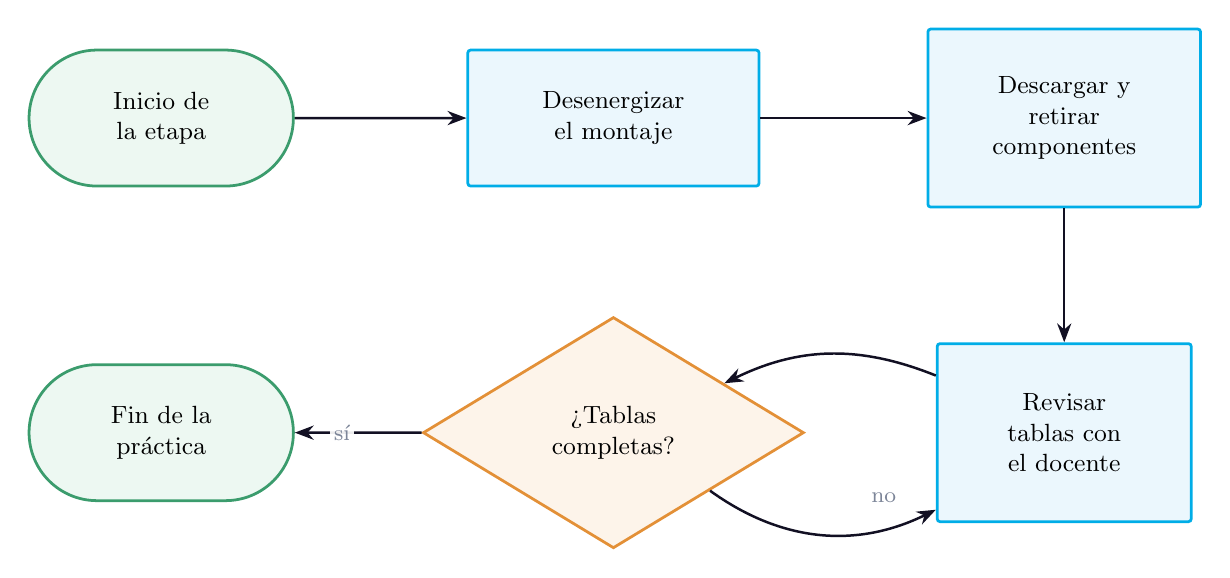
\begin{tikzpicture}[x=1in, y=1in, font=\small]
  % nodos (centro en pulgadas, con el tamano que calcula figuras.py)
  \node[dterminal, minimum width=1.377in, minimum height=0.680in] (n0) at (0.689,-0.445) {Inicio de \\ la etapa};  % ini
  \node[dcaja, minimum width=1.456in, minimum height=0.680in] (n1) at (2.950,-0.445) {Desenergizar \\ el montaje};  % a0
  \node[dcaja, minimum width=1.363in, minimum height=0.890in] (n2) at (5.204,-0.445) {Descargar y \\ retirar \\ componentes};  % a1
  \node[dcaja, minimum width=1.270in, minimum height=0.890in] (n3) at (5.204,-2.018) {Revisar \\ tablas con \\ el docente};  % a2
  \node[ddecision, minimum width=1.905in, minimum height=1.156in] (n4) at (2.950,-2.018) {\textquestiondown{}Tablas \\ completas?};  % dec
  \node[dterminal, minimum width=1.377in, minimum height=0.680in] (n5) at (0.689,-2.018) {Fin de la \\ práctica};  % fin
  % flechas (las de retorno, curvas)
  \draw[dflecha] (n0) -- (n1);
  \draw[dflecha] (n1) -- (n2);
  \draw[dflecha] (n2) -- (n3);
  \draw[dflecha] (n3) to[bend right=24] (n4);
  \draw[dflecha] (n4) -- (n5);
  \draw[dflecha] (n4) to[bend right=31] (n3);
  % rotulos de las flechas (donde los pone el PNG: sin caer sobre un nodo)
  \node[drotulo] at (1.593,-2.018) {sí};
  \node[drotulo] at (4.302,-2.343) {no};
\end{tikzpicture}
\end{adjustbox}
  \caption{Diagrama de flujo de la etapa 4: Desmontaje y cierre}
  \label{fig:flujo-4}
\end{figure}
\begin{pasos}
  \item \textbf{Paso~11:} Apagar el generador de funciones y la fuente, desconectar las puntas del osciloscopio y retirar la alimentación del protoboard. \emph{(aprox.~\SI{3}{\minute})} \textbf{Comprobación:} Ningún indicador de salida debe quedar encendido en el generador ni en la fuente. \textbf{Seguridad:} Desenergizar siempre antes de retirar componentes.
  \item \textbf{Paso~12:} Descargar los condensadores del montaje con la resistencia de descarga, retirar los componentes y devolverlos al kit del grupo con su rótulo. \emph{(aprox.~\SI{4}{\minute})} \textbf{Comprobación:} El kit debe quedar completo, con cada componente en su lugar y con su valor medido anotado.
  \item \textbf{Paso~13:} Revisar con el docente las tablas de registro antes de abandonar el banco. \emph{(aprox.~\SI{3}{\minute})} \textbf{Comprobación:} Las tablas deben estar completas y con unidades; si falta un dato, repetir esa medición antes de desmontar el instrumento.
\end{pasos}

% ---------------------------------------------------------------------
\section{Cuestiones a Resolver}\label{sec:cuestiones}
\begin{enumerate}
  \item \textquestiondown{}Por qué la corriente total es menor que la suma aritmética de las corrientes de rama?
  \item \textquestiondown{}Cómo se compara la corriente total del circuito en paralelo con la del circuito en serie de la semana 4, con los mismos componentes y la misma fuente?
  \item \textquestiondown{}Por qué los ángulos de los circuitos en serie y en paralelo son aproximadamente complementarios?
  \item \textquestiondown{}Qué error introduce el resistor sensor de 10 \ensuremath{\Omega} en la medición de la corriente total?
\end{enumerate}

% ---------------------------------------------------------------------
\section{Análisis de Resultados}\label{sec:analisis}
Calcular con los valores medidos de R y C las corrientes de rama, la corriente total y el ángulo esperados, y compararlos con las mediciones en la tabla de registro, con su diferencia porcentual.
\lineablanco
Dibujar el diagrama fasorial de corrientes con $I_R$ en fase con la tensión e $I_C$ adelantada 90\textdegree{}, y comprobar que su suma vectorial reproduce $I_T$ medida.
% --- Tabla 1: Corrientes y ángulo del circuito RC en paralelo a 1 kHz (7 filas vacías para registrar en el banco) ---
\begin{table}[H]
  \centering
  \caption{Corrientes y ángulo del circuito RC en paralelo a 1 kHz}
  \label{tab:registro-1}
  \begin{tabularx}{\linewidth}{>{\raggedright\arraybackslash}X>{\raggedright\arraybackslash}X>{\raggedright\arraybackslash}X>{\raggedright\arraybackslash}X>{\raggedright\arraybackslash}X}
    \toprule
    \textbf{Magnitud} & \textbf{Calculado} & \textbf{Medido} & \textbf{Unidad} & \textbf{Diferencia (\%)} \\
    \midrule
    \rule{0pt}{0.8cm} & & & & \\
    \cmidrule(lr){1-5}
    \rule{0pt}{0.8cm} & & & & \\
    \cmidrule(lr){1-5}
    \rule{0pt}{0.8cm} & & & & \\
    \cmidrule(lr){1-5}
    \rule{0pt}{0.8cm} & & & & \\
    \cmidrule(lr){1-5}
    \rule{0pt}{0.8cm} & & & & \\
    \cmidrule(lr){1-5}
    \rule{0pt}{0.8cm} & & & & \\
    \cmidrule(lr){1-5}
    \rule{0pt}{0.8cm} & & & & \\
    \bottomrule
  \end{tabularx}
\end{table}

% ---------------------------------------------------------------------
\section{Conclusiones}\label{sec:conclusiones}
Concluir si la ley de corrientes de Kirchhoff se cumple en forma fasorial en el circuito RC en paralelo, explicando las pequeñas diferencias con la resistencia interna del amperímetro y la resolución de los cursores; comparar con el circuito en serie de la semana 4 y relacionarlo con los criterios de medición del RA.
\lineablanco
\begin{itemize}
  \item \textquestiondown{}Qué demuestra la comparación entre la suma aritmética y la fasorial de las corrientes?
  \item \textquestiondown{}Por qué la corriente total se duplicó respecto del circuito en serie?
  \item \textquestiondown{}Qué medición resultó más delicada y por qué?
\end{itemize}

% ---------------------------------------------------------------------
\section{Recomendaciones de Seguridad}\label{sec:seguridad}
\begin{itemize}
  \item Trabajar con el circuito desenergizado mientras se conecta o modifica el montaje; energizar solo después de la revisión del docente.
  \item Descargar los condensadores con una resistencia antes de manipularlos o medirlos, y respetar la polaridad de los electrolíticos: conectado con la polaridad invertida, un electrolítico puede explotar y provocar lesiones \cite{ref1}.
  \item Conectar las tierras de las dos puntas del osciloscopio a un mismo nodo de referencia: unirlas a nodos distintos cortocircuita el elemento que queda entre ellas.
  \item Insertar el amperímetro en serie con la rama solo con el circuito desenergizado y con el instrumento en la función y la escala de corriente; nunca conectarlo en paralelo con la fuente.
\end{itemize}

% ---------------------------------------------------------------------
\section{Bibliografía}\label{sec:bibliografia}
% Las fuentes cargadas se citan en el texto con \cite{refN}; el \nocite del principio fija su orden y \nocite{*} incluye las demás del .bib.
\nocite{*}
\bibliografia

\end{document}
